% ============================================================== QUESTION 2 (part b)
% ------------------------------------------------------------------ 4. What can data fix?
\subsection*{4.\ What Can Data Fix?}
Models B and C each change one thing relative to A; model D changes only the architecture relative to C; D+B (optional) adds symmetry augmentation to D. All were trained with the protocol of \emph{Training and evaluation} (seeds 0 and 1). Symmetry augmentation draws $g\in G$ uniformly per training window (including the identity) and applies it to input and target; speed augmentation draws $k\in\{1,2,3\}$ and then $t$ uniformly from the allowed starts ($14/8/2$).

\Q{Q2.11}{\textbf{Prediction, written before training B, C or D} (verbatim from \texttt{predictions/Q2.11.md}, committed before training B, C or D; no candidate design of D had been trained either).
\begin{quote}\small
Testing the Baseline showed that model A is almost consistent under mirror and rotation ($E_M$ and $E_R$ within about 8\,\% of $E^{(5)}$, $C_M$ and $C_R$ about 8\,\% and 14\,\% of $E^{(5)}$), but that at $2\times$ and $3\times$ its $E^{(2)}$ (0.044, 0.052) is more than twice its $1\times$ value and worse than the all-zero Blank predictor; its reach (8\,px) is below the apparent displacement at $3\times$ (about 10\,px) and borderline at $2\times$ (about 6.6\,px typical, 8+\,px for the fastest digits).\\[2pt]
\textbf{Prediction (three sentences).} Model B (symmetry augmentation) will lower $C_M$, $C_R$, $E_M$ and $E_R$ only slightly, because there is little appearance gap left to close, and will not help at $2\times$ or $3\times$. Model C (speed augmentation, same reach) will fix most of the $2\times$ failure (unfamiliar motion) but will still fail clearly at $3\times$, where the apparent displacement exceeds its 8\,px reach. Model D (reach 16\,px, with speed augmentation) will fix $3\times$ as well, at little or no cost in $1\times$ accuracy.
\end{quote}
\emph{After the fact:} B---right. C---right at $2\times$, \textbf{wrong at $3\times$}: C also fixes most of the $3\times$ failure ($E^{(2)}$ $0.0516\to0.0332$). D---it fixes $3\times$, but only slightly better than C ($0.0320$), and not ``at little cost'' at $1\times$: the cost ($E^{(5)}$ $0.0220\to0.0267$) is already paid by C. The reach I estimated was \emph{not} the main bottleneck (see Q2.13).}

\begin{table}[H]\centering\scriptsize\setlength{\tabcolsep}{2.5pt}
\caption{Models A--D (and optional D+B) on the 1000 test videos, both seeds. $E^{(5)}$, $C_T$, $E_T$ at $1\times$, $t=1$; $E^{(2)}$ at $1\times$, $2\times$, $3\times$. Times: see hardware in the text.}\label{tab:t5}
\begin{tabular}{lrrrrrrrrrrr}\toprule
Model & $E^{(5)}$ & $C_M$ & $E_M$ & $C_R$ & $E_R$ & $E^{(2)}_{1\times}$ & $E^{(2)}_{2\times}$ & $E^{(2)}_{3\times}$ & Params & s/epoch & Infer. (s) \\ \midrule
A baseline (mean) & 0.0220 & 0.00177 & 0.0226 & 0.00300 & 0.0237 & 0.0187 & 0.0444 & 0.0516 & 480{,}784 & 13.6 & 0.586 \\
\quad seed 0 & 0.0222 & 0.00162 & 0.0228 & 0.00262 & 0.0237 & 0.0189 & 0.0433 & 0.0508 & 480{,}784 & 13.6 & 0.596 \\
\quad seed 1 & 0.0217 & 0.00192 & 0.0224 & 0.00338 & 0.0237 & 0.0185 & 0.0455 & 0.0524 & 480{,}784 & 13.5 & 0.576 \\
\midrule
B +sym.\ aug. (mean) & 0.0223 & 0.00128 & 0.0223 & 0.00153 & 0.0223 & 0.0187 & 0.0447 & 0.0509 & 480{,}784 & 23.1 & 0.573 \\
\quad seed 0 & 0.0230 & 0.00128 & 0.0231 & 0.00163 & 0.0229 & 0.0192 & 0.0450 & 0.0520 & 480{,}784 & 23.1 & 0.575 \\
\quad seed 1 & 0.0216 & 0.00128 & 0.0216 & 0.00144 & 0.0216 & 0.0182 & 0.0444 & 0.0498 & 480{,}784 & 23.1 & 0.572 \\
\midrule
C +speed aug. (mean) & 0.0269 & 0.00109 & 0.0271 & 0.00206 & 0.0279 & 0.0234 & 0.0289 & 0.0332 & 480{,}784 & 14.0 & 0.574 \\
\quad seed 0 & 0.0274 & 8.76e-04 & 0.0277 & 0.00166 & 0.0283 & 0.0240 & 0.0295 & 0.0335 & 480{,}784 & 14.0 & 0.568 \\
\quad seed 1 & 0.0263 & 0.00130 & 0.0265 & 0.00245 & 0.0274 & 0.0228 & 0.0283 & 0.0330 & 480{,}784 & 14.0 & 0.579 \\
\midrule
D larger reach (mean) & 0.0267 & 0.00109 & 0.0269 & 0.00235 & 0.0278 & 0.0238 & 0.0282 & 0.0320 & 603{,}088 & 20.8 & 0.648 \\
\quad seed 0 & 0.0267 & 0.00129 & 0.0269 & 0.00272 & 0.0279 & 0.0238 & 0.0282 & 0.0320 & 603{,}088 & 18.8 & 0.650 \\
\quad seed 1 & 0.0267 & 8.93e-04 & 0.0269 & 0.00199 & 0.0278 & 0.0239 & 0.0283 & 0.0319 & 603{,}088 & 22.8 & 0.646 \\
\midrule
D+B (mean) & 0.0276 & 4.55e-04 & 0.0277 & 4.78e-04 & 0.0277 & 0.0247 & 0.0295 & 0.0330 & 603{,}088 & 33.0 & 0.657 \\
\quad seed 0 & 0.0275 & 5.96e-04 & 0.0275 & 5.68e-04 & 0.0276 & 0.0246 & 0.0295 & 0.0328 & 603{,}088 & 35.7 & 0.651 \\
\quad seed 1 & 0.0278 & 3.15e-04 & 0.0278 & 3.88e-04 & 0.0278 & 0.0249 & 0.0296 & 0.0332 & 603{,}088 & 30.2 & 0.663 \\
\midrule
Copy-last & 0.0641 & 0 & 0.0641 & 0 & 0.0641 & 0.0548 & 0.0661 & 0.0703 & 0 & -- & 1.07e-04 \\
\bottomrule\end{tabular}
\end{table}
{\footnotesize\emph{Timing note.} Times are the logged means over the 30 epochs and the timed inference of the final weights. Some logged epochs of D (seed 0) and D+B (seed 1) were up to $2\times$ faster than the rest (GPU/WSL power-state or clock changes during that period), so I also re-timed all five architectures in a controlled run (idle GPU, seed 0, mean of epochs 2--4): A $10.9$\,s, B $17.1$\,s, C $10.7$\,s, D $14.5$\,s, D+B $20.5$\,s per epoch; the ordering (augmentation overhead of the per-sample symmetry loop; D's dilated, wider layers) is the same as in the table. The inference times of A, B, C are equal ($\approx0.58$\,s for 1000 videos) because they share the architecture; D's is $\approx0.65$\,s.}\par\medskip

\Q{Q2.12}{\textbf{Model D} is the same 9-step free-running ConvLSTM as A (patch 4, two layers, input/output shapes, no teacher forcing, same training protocol), with a different spatial configuration: hidden width $72$ (instead of 64) and a \emph{dilated} second layer: layer~1 is a $3\times3$ convolution (dilation 1), layer~2 a $3\times3$ convolution with \textbf{dilation 2} (zero padding 2 keeps the $16\times16$ size). It has $603{,}088$ trainable parameters ($1.25\times$ A; limit $721{,}176$). The design was chosen on the \emph{validation split only} from six candidates (dilated, 5$\times$5-kernel, wider and patch-8 variants; all within the parameter limit and with reach $>8$\,px), each trained for 12 epochs with the C protocol (seed 0) and ranked by the pre-declared score mean($E^{(5)}$@$1\times$, $E^{(2)}$@$2\times$, $E^{(2)}$@$3\times$) (\texttt{results/d\_design.json}); this one scored best ($0.0316$ vs.\ $0.0339$ for the runner-up). Caveat: three candidates (d2, d4, d5 in \texttt{results/d\_design.json}) were still on the initial loss plateau after 12 epochs, so the choice partly reflects how quickly a design starts learning.\\[2pt]
\textbf{Reach, same method as Q2.3.} Radius of a dilated $3\times3$ convolution $=d\cdot(k-1)/2$ cells: layer~1 $1$ cell, layer~2 $2$ cells. Longest paths in one step: new input $u_\tau\to$ layer~1 ($1$) $\to$ layer~2 ($2$) $=3$ cells; $h^{(1)}_{\tau-1}\to$ layer~1 ($1$) $\to$ layer~2 ($2$) $=3$ cells; $h^{(2)}_{\tau-1}\to$ layer~2 recurrent ($2$) $=2$ cells; the $1\times1$ convolution, pixel-shuffle and sigmoid add nothing. With one cell $=4$ px the reach is $3\times4=\mathbf{12}$\,px, strictly larger than A's $8$\,px (the offsets $\{-1,0,1\}+\{-2,0,2\}$ cover $-3..3$ without gaps, so no ``checkerboard'' blind spots). Verified numerically with autograd (\texttt{src/reach\_check.py}: $3,3,2$ cells $\Rightarrow$ $12$\,px). Compared with the displacements of Q2.9: $12>10.4$\,px, so D can reach the median digit even at $3\times$ (A could not).}

\Q{Q2.13}{\textbf{Labels (Table~\ref{tab:t5}, Table~S1; means of seeds).}
\begin{itemize}[leftmargin=*,itemsep=1pt,topsep=2pt]
\item \emph{Appearance} (mirror/rotation, $1\times$): small in A and removed by B. $E_R-E^{(5)}$: A $0.0017$ (A: $E_R=0.0237$) $\to$ B $-0.0001$ ($E_R=0.0223$); $C_R$: $0.00300\to0.00153$; $C_M$: $0.00177\to0.00128$. Models without symmetry augmentation (C, D) keep a gap ($E_R-E^{(5)}=0.0010$--$0.0012$), B closes it, which is why I attribute it to appearance.
\item \emph{Unfamiliar motion} ($2\times$ and $3\times$): B does not help ($E^{(2)}$ $0.0447$, $0.0509$ vs A's $0.0444$, $0.0516$) but C does: $E^{(2)}_{2\times}$ $0.0444\to0.0289$ ($-35\%$), $E^{(2)}_{3\times}$ $0.0516\to0.0332$ ($-36\%$), and the digits' displacement at $2\times$ rises from $39\%$ (A) to $84\%$ of the truth (Table~S1), at $3\times$ from $22\%$ to $72\%$. Same architecture, same reach, only the training speeds changed: this is the dominant cause, at both speeds.
\item \emph{Architectural reach}: D versus C changes only the architecture: $E^{(2)}_{3\times}$ $0.0332\to0.0320$ ($-3.7\%$, lower in both seeds: C $0.0335, 0.0330$; D $0.0320, 0.0319$), $E^{(2)}_{2\times}$ $0.0289\to0.0282$ ($-2.4\%$); displacement at $3\times$ $72\%\to77\%$. A real but small contribution, mainly at $3\times$, where the true displacement ($10.4$\,px) exceeds A's reach.
\end{itemize}
\textbf{If C still did badly at $3\times$ while D did well} that would show that the failure was \emph{architectural}: more training data cannot carry information further than the architecture allows, because the output at a pixel is a function of a bounded set of input cells (the gradient with respect to anything beyond the reach is exactly zero, as checked numerically) and training can only change how the available paths are weighted, never create new ones. Here it did not happen: C already reaches $72\%$ of the true $3\times$ displacement with its nominal 8\,px reach, so, as Q2.9 anticipated, the nominal reach overstates the true limitation once the network has seen fast motion. That \emph{I predicted otherwise in Q2.11 was wrong}.}

\Q{Q2.14}{\textbf{Yes, there is a cost at $1\times$, and it comes from speed augmentation, not from the architecture.} $E^{(5)}$ at $1\times$: A $0.0220$, B $0.0223$ ($+1.7\%$, within the seed spread $0.0216$--$0.0230$), C $0.0269$ ($+22\%$), D $0.0267$ ($+22\%$); $E^{(2)}$ at $1\times$: A $0.0187$, C $0.0234$ ($+25\%$), D $0.0238$ ($+27\%$). The network now spends its fixed capacity and 30 epochs on three speeds, so it is less sharp at the one it was good at. \textbf{Worth it?} For a forecaster that must work at several speeds, yes: $-36\%/-38\%$ error at $2\times/3\times$ (D) for $+22\%$ at $1\times$; A at $2\times$ and $3\times$ is worse than predicting a blank frame ($0.0426$), whereas C and D beat Blank by about $32\%$ at $2\times$ and $22$--$25\%$ at $3\times$. For a $1\times$-only use case it is not worth it. B is essentially free in accuracy and improves consistency (Q2.15), so yes for B. D costs $\approx1.1\times$ inference time over C and $\approx1.4\times$ epoch time, for $-3$ to $-4\%$ error at $3\times$ and no gain at $1\times$.}

% ------------------------------------------------------------------ 5. Final model
\subsection*{5.\ The Final Model}
\textbf{Why $\bar f$ has $C_M=C_R=0$ exactly.} Let $T\in\{M,R\}\subset G$ and $f$ any forecaster. $G$ is a group, so for fixed $T$ the map $g\mapsto h=gT$ is a bijection of $G$, and $g^{-1}=Th^{-1}$. Then
\[
\bar f(T(X))=\tfrac18\sum_{g}g^{-1}\big(f(gT(X))\big)=\tfrac18\sum_{h}T\,h^{-1}\big(f(h(X))\big)=T\Big(\tfrac18\sum_{h}h^{-1}(f(h(X)))\Big)=T(\bar f(X)),
\]
because $T$ only permutes pixels (a linear map that commutes with the average). Hence $C_T=\mathrm{MSE}(\bar f(T(X)),T(\bar f(X)))=0$ for every $f$, and also $E_T=\mathrm{MSE}(T\bar f(X),T(Y))=E^{(5)}$. In floating point, the inputs $gT(X)$ and $h(X)$ are bitwise identical (pure data movement), so every call of $f$ gives identical outputs, and only the order of the eight summands differs; I accumulate in float64, so the measured $C_M$, $C_R$ are $0$ (to the printed precision: exactly $0.00$).

\textbf{Choice of the final model.} The final model is \textbf{D wrapped as a symmetrised forecaster}. I also trained D+B (optional) and chose between them on the \emph{validation} split with the wrapped forecasters: $E^{(5)}$ $0.0264$ (sym.\ D) vs $0.0272$ (sym.\ D+B) (mean of seeds): D is better, and it is also cheaper to train, so the final model is sym.\ D.

\begin{table}[H]\centering\scriptsize\setlength{\tabcolsep}{2.5pt}
\caption{Symmetrised forecasters $\bar f$ (eq.~7) on the test set. Training time is that of the underlying learned model; inference includes all 8 transformations, forward passes, inverse transformations and averaging.}\label{tab:t6}
\begin{tabular}{lrrrrrrrrrrr}\toprule
Model & $E^{(5)}$ & $C_M$ & $E_M$ & $C_R$ & $E_R$ & $E^{(2)}_{1\times}$ & $E^{(2)}_{2\times}$ & $E^{(2)}_{3\times}$ & Params & s/epoch & Infer. (s) \\ \midrule
sym.\ B (mean) & 0.0217 & 0.00e+00 & 0.0217 & 0.00e+00 & 0.0217 & 0.0183 & 0.0440 & 0.0500 & 480{,}784 & 23.1 & 2.60 \\
\quad seed 0 & 0.0223 & 0.00e+00 & 0.0223 & 0.00e+00 & 0.0223 & 0.0187 & 0.0443 & 0.0511 & 480{,}784 & 23.1 & 2.77 \\
\quad seed 1 & 0.0210 & 0.00e+00 & 0.0210 & 0.00e+00 & 0.0210 & 0.0178 & 0.0437 & 0.0488 & 480{,}784 & 23.1 & 2.44 \\
\midrule
sym.\ D (mean) & 0.0265 & 0.00e+00 & 0.0265 & 0.00e+00 & 0.0265 & 0.0237 & 0.0282 & 0.0318 & 603{,}088 & 20.8 & 3.13 \\
\quad seed 0 & 0.0264 & 0.00e+00 & 0.0264 & 0.00e+00 & 0.0264 & 0.0236 & 0.0281 & 0.0319 & 603{,}088 & 18.8 & 3.08 \\
\quad seed 1 & 0.0267 & 0.00e+00 & 0.0267 & 0.00e+00 & 0.0267 & 0.0239 & 0.0282 & 0.0318 & 603{,}088 & 22.8 & 3.19 \\
\midrule
sym.\ D+B (mean) & 0.0275 & 0.00e+00 & 0.0275 & 0.00e+00 & 0.0275 & 0.0246 & 0.0294 & 0.0329 & 603{,}088 & 33.0 & 3.14 \\
\quad seed 0 & 0.0273 & 0.00e+00 & 0.0273 & 0.00e+00 & 0.0273 & 0.0244 & 0.0294 & 0.0327 & 603{,}088 & 35.7 & 3.09 \\
\quad seed 1 & 0.0276 & 0.00e+00 & 0.0276 & 0.00e+00 & 0.0276 & 0.0248 & 0.0294 & 0.0331 & 603{,}088 & 30.2 & 3.20 \\
\bottomrule\end{tabular}
\end{table}
\begin{figure}[!htbp]\centering
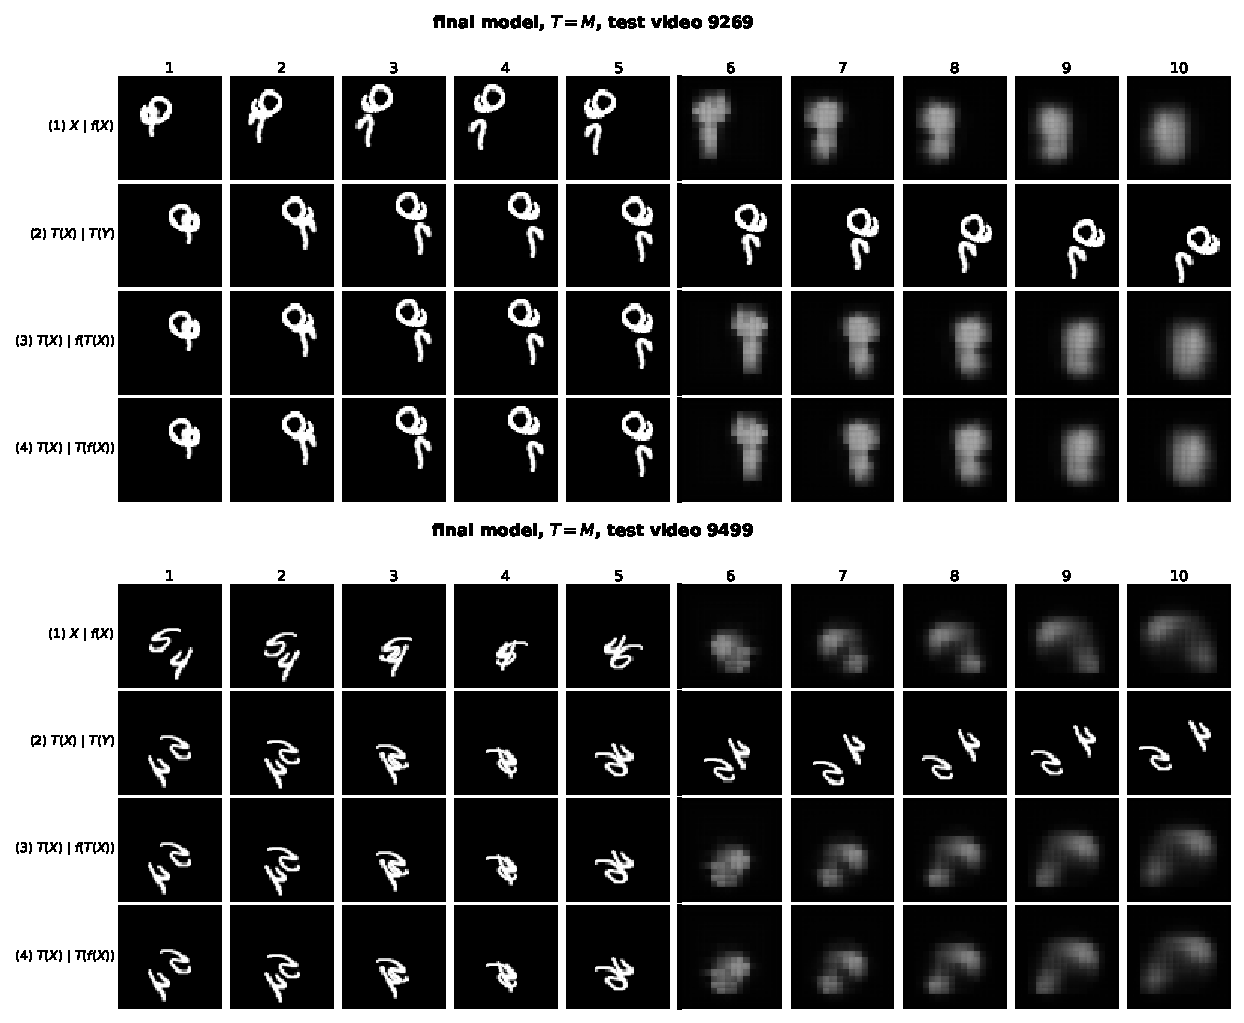
\includegraphics[width=0.88\linewidth]{fig6a_M.pdf}\\[2pt]
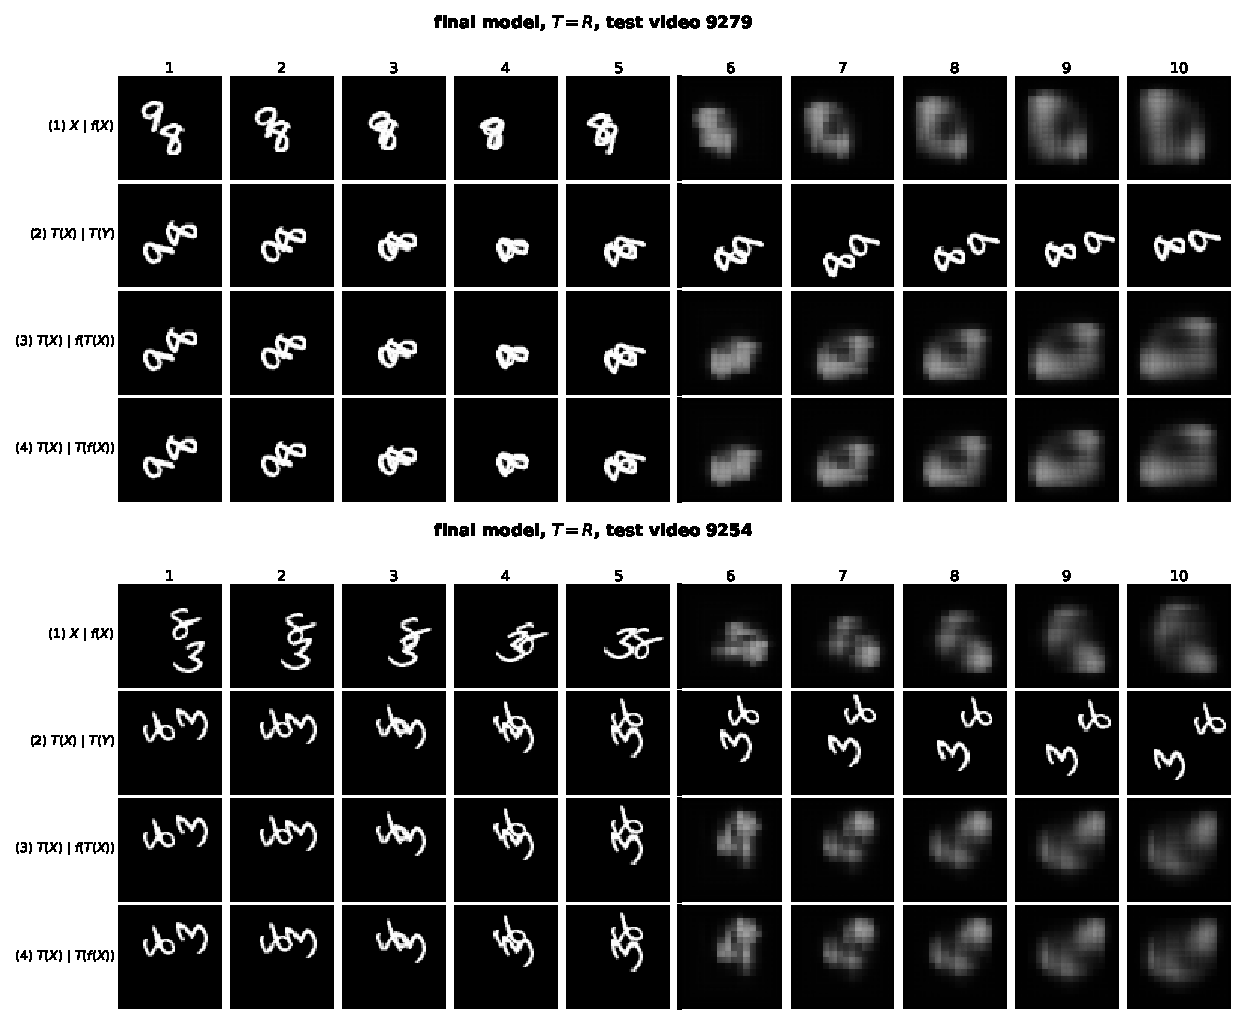
\includegraphics[width=0.88\linewidth]{fig6a_R.pdf}
\caption*{\textbf{Figure 6(a).} Figure 3 repeated with the final model (symmetrised D, seed 0) on exactly the same four test videos (top $T=M$: 9269, 9499; bottom $T=R$: 9279, 9254); rows as in Figure~\ref{fig:f3}. Rows 3 and 4 are identical by construction. GIFs: \texttt{figures/gifs/fig6a\_M\_rank1\_video9269.gif}, \texttt{fig6a\_M\_rank2\_video9499.gif}, \texttt{fig6a\_R\_rank1\_video9279.gif}, \texttt{fig6a\_R\_rank2\_video9254.gif}.}
\end{figure}
\begin{figure}[!htbp]\centering
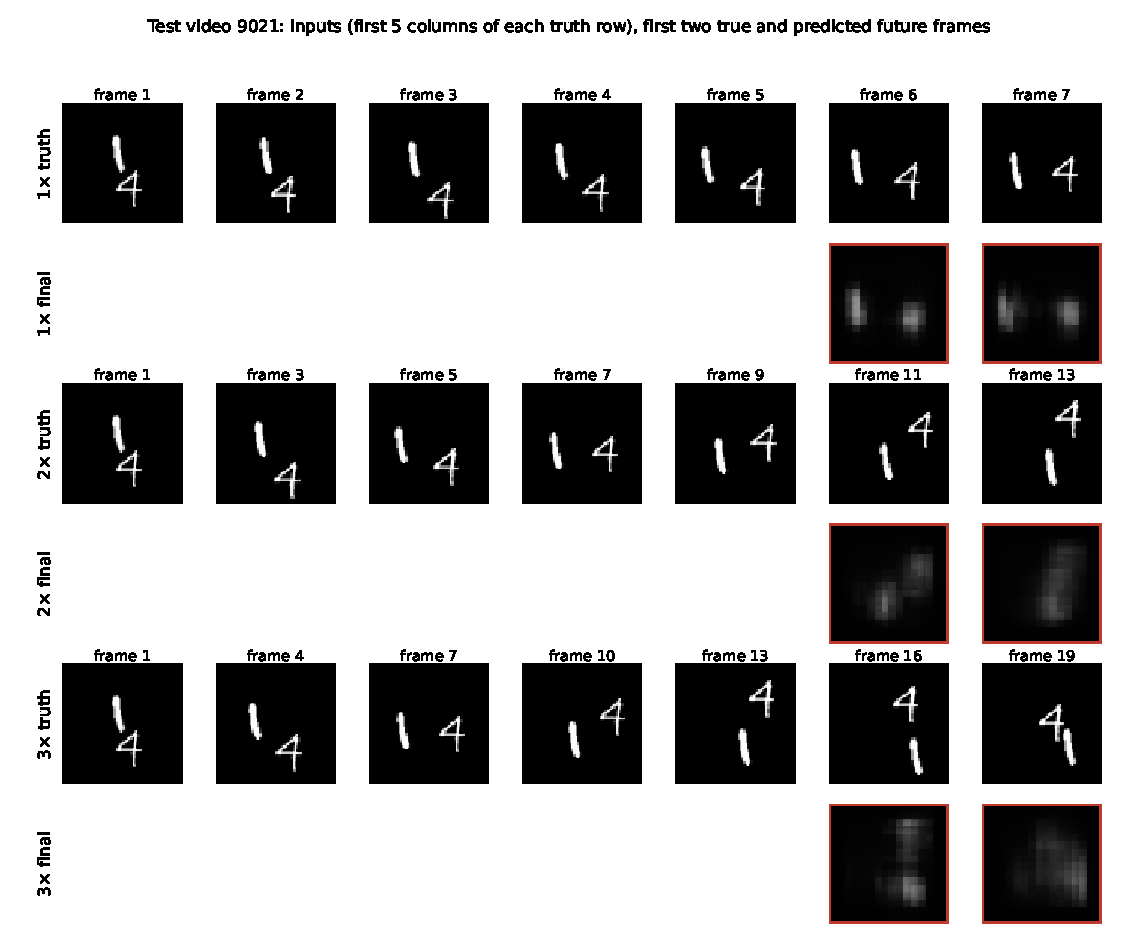
\includegraphics[width=0.93\linewidth]{fig6b_speed.pdf}
\caption*{\textbf{Figure 6(b).} Figure 5 repeated with the final model (symmetrised D, seed 0) on exactly the same test video (9021): inputs, first two true and predicted future frames at $1\times$, $2\times$, $3\times$.}\label{fig:f6b}
\end{figure}
\begin{table}[H]\centering\small
\caption*{\textbf{Table S1} (supplementary). Median centroid displacement (px) of a digit from the last input frame to the first forecast frame at $1\times$, $2\times$, $3\times$ (digits that form separate blobs in both frames; mean over seeds 0, 1 of each model's median; in brackets: median predicted/true per digit). Truth: 3.61, 7.07, 10.44 px.}
\begin{tabular}{lrrr}\toprule
Model & $1\times$ & $2\times$ & $3\times$ \\ \midrule
A (baseline) & 3.36 (96\%) & 2.49 (39\%) & 2.05 (22\%) \\
B (+sym.\ aug.) & 3.40 (97\%) & 2.64 (42\%) & 2.56 (27\%) \\
C (+speed aug.) & 3.23 (93\%) & 5.43 (84\%) & 6.84 (72\%) \\
D (reach 12 px) & 3.32 (96\%) & 5.73 (87\%) & 7.26 (77\%) \\
final: sym.\ D & 3.40 (97\%) & 5.80 (88\%) & 7.15 (76\%) \\
\bottomrule\end{tabular}\end{table}
\begin{table}[H]\centering\small
\caption*{\textbf{Table S2} (supplementary). $E^{(5)}$ (mean over seeds, $1\times$, $t=1$) on forward and on \emph{time-reversed} test videos, and on the 586 test videos whose digits overlap in frames 6--10 versus the other 414.}
\begin{tabular}{lrrrr}\toprule
Model & forward & time-reversed & overlap in 6--10 & no overlap \\ \midrule
A (baseline) & 0.0220 & 0.0219 & 0.0216 & 0.0225 \\
B (+sym.\ aug.) & 0.0223 & 0.0222 & 0.0219 & 0.0230 \\
C (+speed aug.) & 0.0269 & 0.0266 & 0.0259 & 0.0282 \\
D (reach 12 px) & 0.0267 & 0.0265 & 0.0257 & 0.0280 \\
final: sym.\ D & 0.0265 & 0.0264 & 0.0255 & 0.0280 \\
\bottomrule\end{tabular}\end{table}

\Q{Q2.15}{\textbf{Learned (B) versus built-in (symmetrised).} \emph{Consistency:} B reduces the gaps ($C_M$ $0.00177\to0.00128$, $C_R$ $0.00300\to0.00153$) but not to zero; the wrapped models have $C_M=C_R=0$ \emph{exactly}, for any $f$ (proof above). Augmentation only \emph{encourages} the symmetry on the data it saw; averaging \emph{imposes} it, so only the built-in version is exact. \emph{Accuracy on original clips ($1\times$):} sym.\ B $E^{(5)}=0.0217$ vs B $0.0223$ ($-2.8\%$); sym.\ D $0.0265$ vs D $0.0267$ ($-0.6\%$); on transformed clips, $E_M=E_R=E^{(5)}$ for the wrapped models by the identity above (B: $0.0223$/$0.0223$ vs $0.0223$). \emph{Inference cost:} B $0.57$\,s $\to$ sym.\ B $2.60$\,s ($4.5\times$) and D $0.65\to3.13$\,s ($4.8\times$) for 1000 videos (eight forward passes, not exactly $8\times$ because small batches do not saturate the GPU); training cost is unchanged for the wrapper, while B itself already costs $\approx1.6$--$1.7\times$ the training time per epoch. \textbf{When would built-in symmetry hurt?} Averaging eight predictions blurs when the predictions are sharp and the views disagree, i.e.\ when the world is \emph{not} symmetric: a drift or gravity in one direction, orientation-specific appearance that matters for the forecast, or a symmetry that holds only approximately. It did not hurt here: the dynamics (constant velocity, elastic bounces in a square box) are exactly $G$-symmetric and the forecasts are already blurry, so averaging acts like a small ensemble ($-0.6\%$ to $-2.8\%$ error).}

\Q{Q2.16}{\textbf{Video 9279, $T=R$ (Figures~\ref{fig:f3} and 6(a)).} Model A's two views disagreed (rotated input: stalled blob, centroid $0.27$\,px/frame vs truth $1.46$; original: $1.44$). In the final model the disagreement is gone: rows 3 and 4 are identical (centroid gap $0.0$\,px); but it is \emph{not} right: both views move at $0.79$\,px/frame (truth $1.46$), and the forecast's ink grows from $306$ to $480$ (truth $255\to273$), i.e.\ it still under-moves and blurs. Which change fixed what: \emph{symmetrisation} fixed the disagreement (consistency: $C_R=0$); \emph{symmetry augmentation (B)} reduced the stall in the rotated view ($0.27\to1.19$\,px/frame, B seed 0) --- so the stall was mostly appearance; \emph{speed augmentation and reach (C, D)} did not change this $1\times$ video ($D$: $0.78/1.11$, i.e.\ no improvement), and the remaining under-motion is the general $1\times$ cost of Q2.14 (D, C are less sharp at $1\times$ than A). In short: consistency repaired, accuracy on this overlap video not.}

\Q{Q2.17}{\textbf{Final verdict (150 words).} \emph{Partly.} Evidence for motion rather than memory: exact $G$-consistency ($C_M=C_R=0$, $E_M=E_R=E^{(5)}=0.0265$); the same error on \emph{time-reversed} videos ($0.0264$ vs $0.0265$, Table~S2); at $2\times$/$3\times$ the digits travel $88\%$/$76\%$ of the true distance (A: $39\%$/$22\%$) and $E^{(2)}$ falls to $0.0282$/$0.0318$ (A $0.0444$/$0.0516$). Against: forecasts stay blurry ($0.0265$, only $38\%$ below Blank) and under-move at $3\times$. \emph{A skeptic would be convinced} by sharp forecasts with the right displacement at speeds \emph{outside} the training set (e.g.\ non-integer or faster). \emph{Test not passed:} tracking digit identity through overlaps --- Figure~6a (video 9279) is still blurred and slow.}
